% Assignment 1
\question Explain the overheads and difficulties relating to fault-tolerant routing in the two contexts of: pre-building routes and storing them in routing tables at the nodes; or building routes on-the-fly.
\begin{solution}
  When prebuilding routes, we can only deal with faults at the time of building routes. After this point, if a node fails it may still be included in a route as when the routes were built it was assumed to be working. This makes prebuilding routes a typically ineffective method for fault-tolerant routing, unless we frequently recalculate the routes.

  When calculating routes on-the-fly, we are able to work around faults and route regardless. However, this requires a solid description of the network; that is, each node needs to have an understanding of its neighbours and whether they are faulty. Additionally, this may add significantly to the computation time when sending a message. 
  % todo
  % Prebuilding routes:
  % \begin{enumerate}
  %   \item a pre-built route may traverse a node that has failed, making it invalid.
  %   \item trade-off on memory to computation
  % \end{enumerate}
  % On the fly:
  % \begin{enumerate}
  %   \item increased overhead of calculating routes
  %   \item can work around failed nodes
  %   \item requires description of graph
  % \end{enumerate}
\end{solution}

\question The 4-dimensional hypercube $Q_4$ is detailed on slide 15 of Lecture 1. It takes 4 bits to store the name of a node.
\begin{parts}
  \part If there is a table at each node $u \in \{0, 1\}^4$ with an entry for each destination and with the entry being a full path from $u$ to the destination, how many bits are required to store all of the entries in the table?

  [You may assume that for each entry, the source need not be stored but the rest of the path, including the destination, needs to be stored.]
  \begin{solution}
    We assume dimension-ordered routing. We have
    \[ b_\text{total} = \sum_{n \in N \setminus \{u\}} D(u, n) \cdot b \]
    where $D(u,n)$ denotes the distance between $u$ and $n$, and $b$ is the number of bits required to store a node. 
    We have 4 vertices of distance 1 away, 6 of distance 2 away, and 4 of distance 3 away, and 1 of distance 4 away. Thus
    \[ b_\text{total} = (4)(1b) + (6)(2b) + (4)(3b) + (1)(4b) = 32b. \]
    As a node is an element of $\{0,1\}^4$, then $b = 4$. Thus 
    \[ b_\text{total} = \SI{128}{\bit}. \]
  \end{solution}

  \part If there is a table at each node $u \in \{0,1\}^4$ with an entry for each destination and with the entry being only the next node on a path from $u$ to the destination, how many bits does it take to store all of the entries in the table? 
  \begin{solution}
    Following a similar reasoning to part (a), we get the following.
    \[ b_\text{total} = (2^4 - 1)(b) = \SI{60}{\bit} \]
  \end{solution}

  \part Develop a coding scheme so as to reduce the total number of bits required to store the table in ($b$) as much as you can and state how many storage bits you require. 
  \begin{solution}
    For each node, we store a 2 digit binary number $b \in \{0,1\}^2$ which corresponds to the bit to flip to get to the next node in the path. For example, if $b = (0,0)$ we flip the first bit to get to the next neighbour. If $b = (1,1)$, we flip the fourth bit to get to the next neighbour. This requires $(2^4 - 1) \cdot 2 = 30$ bits per node. 
  \end{solution}
\end{parts}

\question 
\begin{parts}
  \part Any graph can always be described by its adjacency matrix. However, in the context of interconnection networks where the number of nodes might be a million, a concise algebraic description is necessary. Give concise algebraic descriptions of the two interconnection network topologies that are natural generalizations of those in Fig. 1 to $n$ nodes where $n$ is divisible by $2$ but not by $4$.
  \begin{solution}
    Circulent graph:
    \begin{align*}
      V &= \{v_0, \ldots, v_{n-1}\} \\
      E &= \{(v_{i \bmod n}, v_{i+1 \bmod n}): i \in \{0, \ldots, n-1\}\} \;\cup \tag{1} \\
        &\qquad \{(v_{i \bmod n}, v_{i + \frac n2 \bmod n}): i \in \{0,\ldots, n-1\}\}. \tag{2}
    \end{align*}
    Here the edges defined in (1) are the outside cycle and (2) are the edges between antipodal points.
    Peterson graph:
    \begin{align*}
      V &= \{v_0, \ldots, v_{n-1}\} \\
      E &= \{(v_{2i \bmod n}, v_{2i+2 \bmod n}): i \in \{0, \ldots, n/2-1\}\} \;\cup \tag{3} \\
        &\qquad \{(v_{2i+1 \bmod n}, v_{2i+5 \bmod n}): i \in \{0, \ldots, n/2-1\}\} \;\cup \tag{4} \\
        &\qquad \{(v_{2i\bmod n}, v_{2i+1 \bmod n}): i \in \{0, \ldots, n/2-1\}\} \tag{5}
    \end{align*}
    (3) defines the cycle on the outside of the graph, (4) defines the graph contained within the cycle, and (5) corresponds to the connections between the cycle and the center. 
  \end{solution}

  \part Suppose that in the two interconnection network topologies in Fig. 1, every channel has bandwidth $b$ \si{\bit\per\second}. Suppose that node $0$ in each topology needs to send a message of $b$ bits to every other node where these messages are all distinct; this is called a \emph{single-node scatter}. For each interconnection network, explain whether this can be accomplished in 3 seconds. 
  \begin{solution}
    This is possible in both graphs, broadcast schedule below.
    \begin{enumerate}
      \item Let $m_i$ be the message sent by $0$ to node $i \in \{1, \ldots, 9\}$. The packets follow the following routes:
      \begin{center}
        \begin{tabular}{cl}
          \toprule
          Message & Route \\
          \midrule
          $m_1$ & $0 \to 1$ \\
          $m_2$ & $0 \to 1 \to 2$ \\
          $m_3$ & $0 \to 1 \to 2 \to 3$ \\
          $m_4$ & $0 \to 5 \to 4$ \\
          $m_5$ & $0 \to 5$ \\
          $m_6$ & $0 \to 5 \to 6$ \\
          $m_7$ & $0 \to 9 \to 8 \to 7$ \\
          $m_8$ & $0 \to 9 \to 8$ \\
          $m_9$ & $0 \to 9$ \\
          \bottomrule
        \end{tabular}
      \end{center}
        Then we have the following schedule.
        \begin{enumerate}
          \item At time step 1, we send:
          \begin{enumerate}
            \item $m_3$ from 0 to 1,
            \item $m_6$ from 0 to 5,
            \item $m_7$ from 0 to 9.
          \end{enumerate}
          \item At time step 2, we send
          \begin{enumerate}
            \item $m_2$ from 0 to 1,
            \item $m_3$ from 1 to 2,
            \item $m_4$ from 0 to 5,
            \item $m_6$ from 5 to 6 (arrived),
            \item $m_7$ from 9 to 8,
            \item $m_8$ from 0 to 9.
          \end{enumerate}
          \item At time step 3, we send
          \begin{enumerate}
            \item $m_1$ from 0 to 1 (arrived),
            \item $m_2$ from 1 to 2 (arrived),
            \item $m_3$ from 2 to 3 (arrived,
            \item $m_4$ from 5 to 4 (arrived,
            \item $m_5$ from 0 to 5 (arrived),
            \item $m_7$ from 8 to 7 (arrived,
            \item $m_8$ from 9 to 8 (arrived),
            \item $m_9$ from 0 to 9 (arrived).
          \end{enumerate}
        \end{enumerate}

      \item Let $m_i$ be the message sent by $0$ to node $i \in \{1, \ldots, 9\}$. We construct the following routes.
      \begin{center}
        \begin{tabular}{cl}
          \toprule
          Message & Route \\
          \midrule
          $m_1$ & $0 \to 1$ \\
          $m_2$ & $0 \to 2$ \\
          $m_3$ & $0 \to 2 \to 3$ \\
          $m_4$ & $0 \to 2 \to 4$ \\
          $m_5$ & $0 \to 1 \to 5$ \\
          $m_6$ & $0 \to 8 \to 6$ \\
          $m_7$ & $0 \to 1 \to 7$ \\
          $m_8$ & $0 \to 8$ \\
          $m_9$ & $0 \to 8 \to 9$ \\
          \bottomrule
        \end{tabular}
      \end{center}
      We have the following schedule.
      \begin{enumerate}
        \item At time step 1, we send:
        \begin{enumerate}
          \item $m_4$ from 0 to 2,
          \item $m_6$ from 0 to 8,
          \item $m_7$ from 0 to 1.
        \end{enumerate}
        \item At time step 2, we send:
        \begin{enumerate}
          \item $m_3$ from 0 to 2,
          \item $m_4$ from 2 to 4 (arrived),
          \item $m_5$ from 0 to 1,
          \item $m_6$ from 8 to 6 (arrived),
          \item $m_7$ from 1 to 7 (arrived),
          \item $m_9$ from 0 to 8.
        \end{enumerate}
        \item At time step 3, we send:
        \begin{enumerate}
          \item $m_1$ from 0 to 1 (arrived),
          \item $m_2$ from 0 to 2 (arrived),
          \item $m_3$ from 2 to 3 (arrived),
          \item $m_5$ from 1 to 5 (arrived),
          \item $m_8$ from 0 to 8 (arrived). 
        \end{enumerate}
      \end{enumerate}
    \end{enumerate}
  \end{solution}

  \part Suppose that in case ($b$) all messages are identical; that is, node $0$ wishes to send the same message of $b$ bits to every other node. This is called a \emph{single-node broadcast}. For each interconnection network in Fig. 1, explain whether this single-node broadcast can be accomplished in $2$ seconds. 
  \begin{solution}
    The diameter of the circulent graph is 3 (path $0 \to 5 \to 4 \to 3$ is minimal), thus a single-node broadcast is not possible. However, it is possible for the Peterson graph. Take the routes mentioned in (b).
    \begin{center}
        \begin{tabular}{cl}
          \toprule
          Message & Route \\
          \midrule
          $m_1$ & $0 \to 1$ \\
          $m_2$ & $0 \to 2$ \\
          $m_3$ & $0 \to 2 \to 3$ \\
          $m_4$ & $0 \to 2 \to 4$ \\
          $m_5$ & $0 \to 1 \to 5$ \\
          $m_6$ & $0 \to 8 \to 6$ \\
          $m_7$ & $0 \to 1 \to 7$ \\
          $m_8$ & $0 \to 8$ \\
          $m_9$ & $0 \to 8 \to 9$ \\
          \bottomrule
        \end{tabular}
      \end{center}
      All routes have length of at most 2, so we can just flood the packet at each node and ignore the incoming packet if you have already received it. 
  \end{solution}

  \part Suppose that a \emph{total exchange} is required; that is, every node needs to send a message to every other node and all messages are different. For each interconnection network in Fig. 1, devise a routing whereby there is a path from every node to every other node and calculate the load on every channel; that is, for each channel, the number of paths using the channel.
  \begin{solution}
    \begin{enumerate}
      \item Circulent graph: consider the following image.
      \begin{center}
        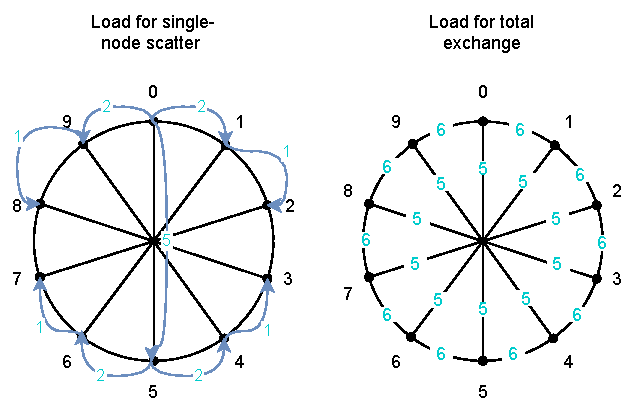
\includegraphics[width=0.8\textwidth]{q3-d-1}
      \end{center}
      This depicts the following routes from node $0$ to every other node.
      \begin{center}
        \begin{tabular}{cl}
          \toprule
          Destination & Route \\
          \midrule
          1 & $0 \to 1$ \\
          2 & $0 \to 1 \to 2$ \\
          3 & $0 \to 5 \to 4 \to 3$ \\
          4 & $0 \to 5 \to 4$ \\
          5 & $0 \to 5$ \\
          6 & $0 \to 5 \to 6$ \\
          7 & $0 \to 5 \to 6 \to 7$ \\
          8 & $0 \to 9 \to 8$ \\
          9 & $0 \to 9$ \\
          \bottomrule
        \end{tabular}
      \end{center}
      As the circulent is node-symmetric by rotational symmetry of order 10, we can just rotate our routes to every node and get the loads as displayed in the image above. 

      \item Peterson graph: consider the following image.
      \begin{center}
        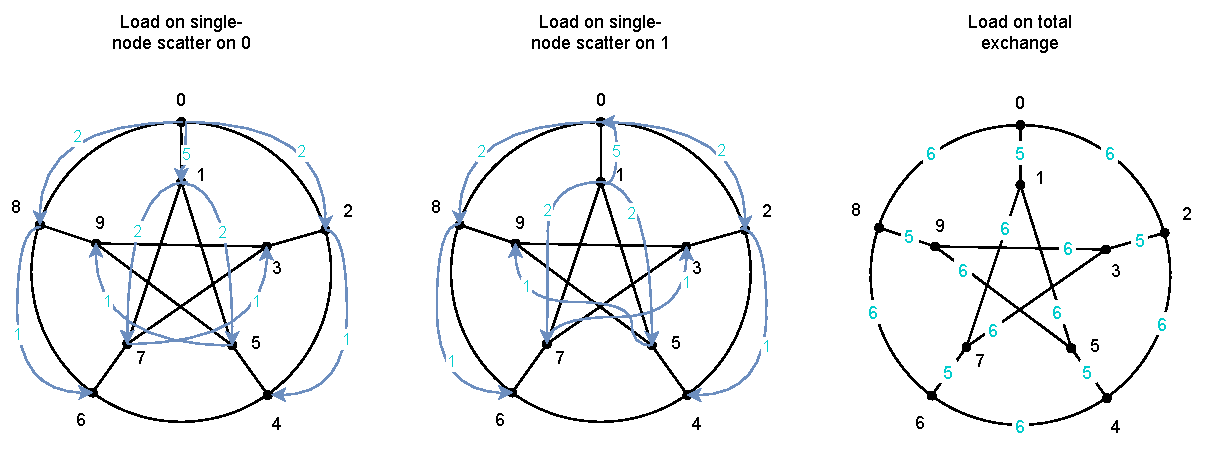
\includegraphics[width=0.95\textwidth]{q3-d-2}
      \end{center}
      Now, the Peterson graph is not node-symmetric; however, it does has rotational symmetry of order 5. Through rotation of $2\pi/5$, we have 2 \emph{connected components} that we can reach. Namely, the odd nodes and the even nodes. Thus, finding a route for $0$ and $1$ is enough to generate both components.
      \begin{center}
        \begin{tabular}{ccl}
          \toprule
          Source & Destination & Route \\
          \midrule
          0 & 1 & $0 \to 1$ \\
          0 & 2 & $0 \to 2$ \\
          0 & 3 & $0 \to 1 \to 7 \to 3$ \\
          0 & 4 & $0 \to 2 \to 4$ \\
          0 & 5 & $0 \to 1 \to 5$ \\
          0 & 6 & $0 \to 8 \to 6$ \\
          0 & 7 & $0 \to 1 \to 7$ \\
          0 & 8 & $0 \to 8$ \\
          0 & 9 & $0 \to 1 \to 5 \to 9$ \\
          1 & 0 & $1 \to 0$ \\
          1 & 2 & $1 \to 0 \to 2$ \\
          1 & 3 & $1 \to 7 \to 3$ \\
          1 & 4 & $1 \to 0 \to 2 \to 4$ \\
          1 & 5 & $1 \to 5$ \\
          1 & 6 & $1 \to 0 \to 8 \to 6$ \\
          1 & 7 & $1 \to 7$ \\
          1 & 8 & $1 \to 0 \to 8$ \\
          1 & 9 & $1 \to 5 \to 9$ \\
          \bottomrule
        \end{tabular}
      \end{center}
      We can similarly rotate the routes for the odd numbered nodes and the routes for the even numbered nodes around the graph to get our final load, as displayed in the image above. 
    \end{enumerate}
  \end{solution}
\end{parts}
\begin{figure}
  \centering
  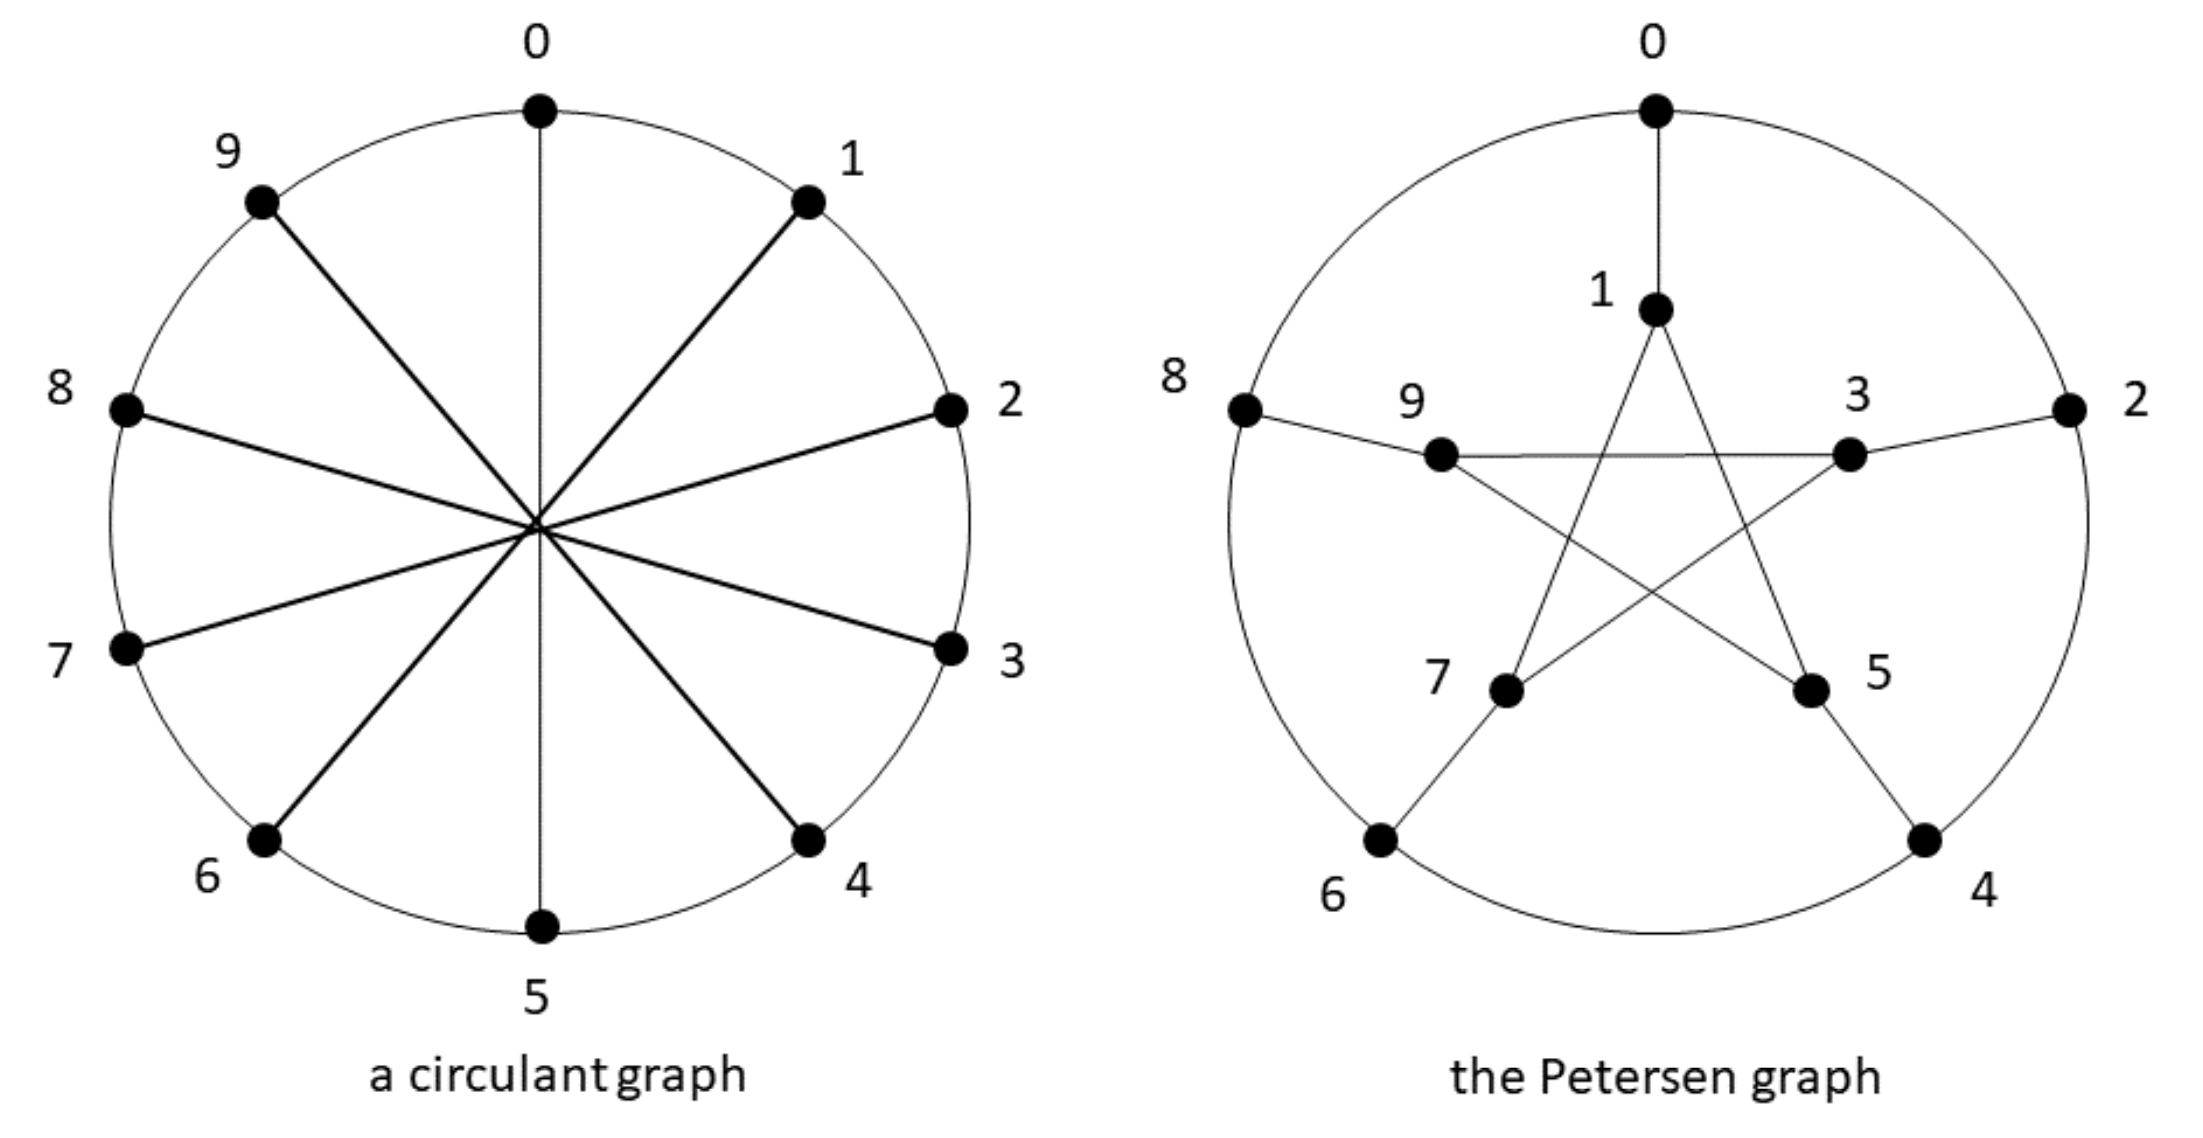
\includegraphics[width=0.5\textwidth]{fig-1}
  \caption{A circulant graph and the Petersen graph.}
\end{figure}  